
\documentclass{article}

\usepackage{fancyhdr}
\usepackage{enumerate}
\usepackage{amsmath}
\usepackage{amsfonts}
\usepackage{amssymb}
\newcommand\tab[1][1cm]{\hspace*{#1}}
\usepackage{tikz}
\usetikzlibrary{arrows,automata}
\usepackage{graphicx}
\usepackage{grffile}


\usepackage{tikz}
\usetikzlibrary{arrows,automata}
\usepackage{graphicx}
\usepackage{grffile}

%
% Basic Document Settings
%

\topmargin=-0.45in
\evensidemargin=0in
\oddsidemargin=0in
\textwidth=6.5in
\textheight=9.0in
\headsep=0.25in

\linespread{1.1}

\pagestyle{fancy}
\lhead{\hmwkAuthorName}
\rhead{\hmwkClass: \hmwkTitle}
\cfoot{\thepage}

\renewcommand\headrulewidth{0.4pt}
\renewcommand\footrulewidth{0.4pt}

\setlength\parindent{0pt}

%
% Homework Details
%   - Title
%   - Due date
%   - Class
%   - Section/Time
%   - Instructor
%   - Author
%

\newcommand{\hmwkTitle}{Homework\ \#4}
\newcommand{\hmwkDueDate}{April 12, 2017}
\newcommand{\hmwkClass}{Design \& Analysis of Algorithms - 344}
\newcommand{\hmwkClassTime}{Section \#2}
\newcommand{\hmwkClassInstructor}{Professor Dr. Kalantari}
\newcommand{\hmwkAuthorName}{\textbf{Douglas Rudolph, Mustufa Hussain}}

%
% Title Page
%

\title{
    \vspace{2in}
    \textmd{\textbf{\hmwkClass:\ \hmwkTitle}}\\
    \normalsize\vspace{0.1in}\small{Due\ on\ \hmwkDueDate\ at 11:59pm}\\
    \vspace{0.1in}\large{\textit{\hmwkClassInstructor\ \hmwkClassTime}}
    \vspace{3in}
}

\author{\hmwkAuthorName}
\date{}

\setlength\parskip{\baselineskip}

\begin{document}
\maketitle
\pagebreak

\textbf{Problem 1} Determine of the following system of inequalities has a feasible solution.
\begin{center}
	\begin{tabular}{c c c c}
		$x_4 - x_2$ &$\leq$ &$-2$ \\
		$x_1 - x_3$ &$\leq$ &$3$ \\
		$x_5 - x_4$ &$\leq$ &$-4$ \\
		$x_3 - x_2$ &$\leq$ &$2$ \\
		$x_2 - x_1$ &$\leq$ &$8$ \\
		$x_4 - x_3$ &$\leq$ &$1$ \\
		$x_1 - x_5$ &$\leq$ &$-3$ \\
	\end{tabular}
\end{center}
If it has no solution can you change −2 in the first inequality to a number so that the system will be feasible? And what would be the smallest such value to change it to so that the system becomes feasible.
Here is the graph that corresponds to the above system: \\
\begin{center}
		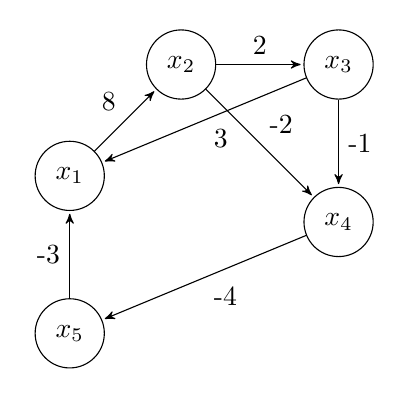
\begin{tikzpicture}[>=stealth',shorten >=1pt,auto,node distance=2cm]
  			\node[state]  (x1) []           {$x_1$};
  			\node[state]             (x2) [above right of=x1]  {$x_2$};
            \node[state]             (x3) [right of=x2]  {$x_3$};
            \node[state]             (x4) [below of=x3]  {$x_4$};
            \node[state]             (x5) [below of=x1]  {$x_5$};


  			\path[->] 
                     (x1) edge node {8} (x2)
                     (x2) edge node {2} (x3)
                     (x3) edge node {-1} (x4)
                     (x4) edge node {-4} (x5)
                     (x5) edge node {-3} (x1)
                     (x3) edge node {3} (x1)
                     (x2) edge node {-2} (x4);
        	         
            	 		
		\end{tikzpicture}
	\end{center}
    
We run the Bellman-Ford on the graph above starting from $x_1$. Note that () indicates a tentative distance. \\
The graph is initialized as such: \\
\begin{center}
		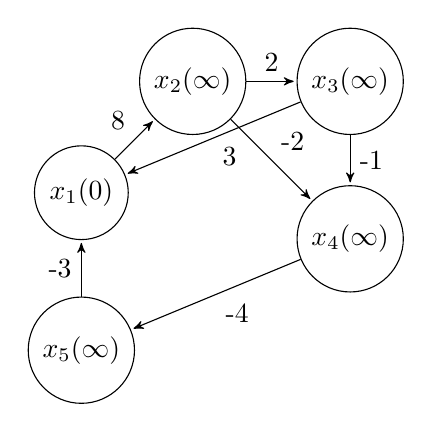
\begin{tikzpicture}[>=stealth',shorten >=1pt,auto,node distance=2cm]
  			\node[state]  (x1) []           {$x_1$(0)};
  			\node[state]             (x2) [above right of=x1]  {$x_2$($\infty$)};
            \node[state]             (x3) [right of=x2]  {$x_3$($\infty$)};
            \node[state]             (x4) [below of=x3]  {$x_4$($\infty$)};
            \node[state]             (x5) [below of=x1]  {$x_5$($\infty$)};


  			\path[->] 
                     (x1) edge node {8} (x2)
                     (x2) edge node {2} (x3)
                     (x3) edge node {-1} (x4)
                     (x4) edge node {-4} (x5)
                     (x5) edge node {-3} (x1)
                     (x3) edge node {3} (x1)
                     (x2) edge node {-2} (x4);
        	         
            	 		
		\end{tikzpicture}
	\end{center}
    
After the first pass:    
\begin{center}
		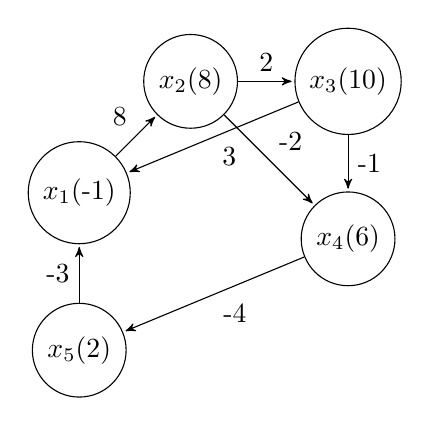
\begin{tikzpicture}[>=stealth',shorten >=1pt,auto,node distance=2cm]
  			\node[state]  (x1) []           {$x_1$(-1)};
  			\node[state]             (x2) [above right of=x1]  {$x_2$(8)};
            \node[state]             (x3) [right of=x2]  {$x_3$(10)};
            \node[state]             (x4) [below of=x3]  {$x_4$(6)};
            \node[state]             (x5) [below of=x1]  {$x_5$(2)};


  			\path[->] 
                     (x1) edge node {8} (x2)
                     (x2) edge node {2} (x3)
                     (x3) edge node [thin]{-1} (x4)
                     (x4) edge node {-4} (x5)
                     (x5) edge node {-3} (x1)
                     (x3) edge node {3} (x1)
                     (x2) edge node {-2} (x4);
        	         
            	 		
		\end{tikzpicture}
	\end{center}
    
After the second pass:    
\begin{center}
		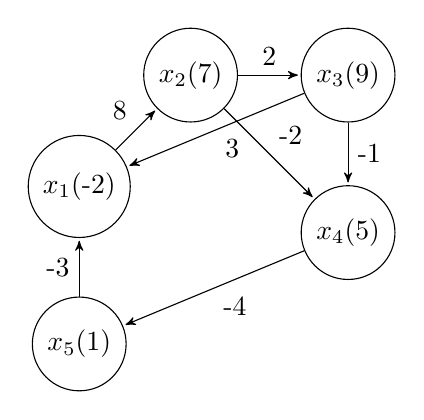
\begin{tikzpicture}[>=stealth',shorten >=1pt,auto,node distance=2cm]
  			\node[state]  (x1) []           {$x_1$(-2)};
  			\node[state]             (x2) [above right of=x1]  {$x_2$(7)};
            \node[state]             (x3) [right of=x2]  {$x_3$(9)};
            \node[state]             (x4) [below of=x3]  {$x_4$(5)};
            \node[state]             (x5) [below of=x1]  {$x_5$(1)};


  			\path[->] 
                     (x1) edge node {8} (x2)
                     (x2) edge node {2} (x3)
                     (x3) edge node {-1} (x4)
                     (x4) edge node {-4} (x5)
                     (x5) edge node {-3} (x1)
                     (x3) edge node {3} (x1)
                     (x2) edge node {-2} (x4);
        	         
            	 		
		\end{tikzpicture}
	\end{center}
    
After the third pass:    
\begin{center}
		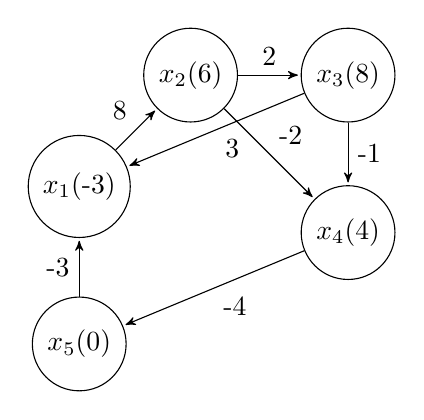
\begin{tikzpicture}[>=stealth',shorten >=1pt,auto,node distance=2cm]
  			\node[state]  (x1) []           {$x_1$(-3)};
  			\node[state]             (x2) [above right of=x1]  {$x_2$(6)};
            \node[state]             (x3) [right of=x2]  {$x_3$(8)};
            \node[state]             (x4) [below of=x3]  {$x_4$(4)};
            \node[state]             (x5) [below of=x1]  {$x_5$(0)};


  			\path[->] 
                     (x1) edge node {8} (x2)
                     (x2) edge node {2} (x3)
                     (x3) edge node {-1} (x4)
                     (x4) edge node {-4} (x5)
                     (x5) edge node {-3} (x1)
                     (x3) edge node {3} (x1)
                     (x2) edge node {-2} (x4);
        	         
            	 		
		\end{tikzpicture}
	\end{center}
    
    
After the fourth (and final) pass:    
\begin{center}
		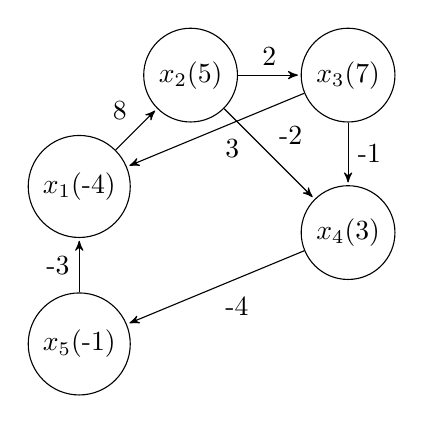
\begin{tikzpicture}[>=stealth',shorten >=1pt,auto,node distance=2cm]
  			\node[state]  (x1) []           {$x_1$(-4)};
  			\node[state]             (x2) [above right of=x1]  {$x_2$(5)};
            \node[state]             (x3) [right of=x2]  {$x_3$(7)};
            \node[state]             (x4) [below of=x3]  {$x_4$(3)};
            \node[state]             (x5) [below of=x1]  {$x_5$(-1)};


  			\path[->] 
                     (x1) edge node {8} (x2)
                     (x2) edge node {2} (x3)
                     (x3) edge node {-1} (x4)
                     (x4) edge node {-4} (x5)
                     (x5) edge node {-3} (x1)
                     (x3) edge node {3} (x1)
                     (x2) edge node {-2} (x4);
        	         
            	 		
		\end{tikzpicture}
	\end{center}

We now check for negative cycles and find that the edge from $x_1$ to $x_2$ satisfies the negative cycle condition (that is, 5 > (8 + -4)). As such, we conclude that this graph has a negative cycle, which implies that the system is infeasible. \\

We see that the negative cycle from $x_1$ to $x_2$ to $x_4$ to $x_5$ and back to $x_1$ has a edge sum of (8 + -2 + -4 + -3) = -1. As such, we can change the edge with -2 (the inequality $x_4 - x_2 \leq -2$) to -1 (that is, the inequality becomes $x_4 - x_2 \leq -1$) so that the edge sum becomes non-negative (8 + -1 + -4 + -3 = 0).
\newpage

\textbf{Problem 2}. 
Given 4 matrices, $A1, . . . , A4$, where $Ai$ is $m_{i - 1}$ x $m_{i}$ matrix, $i = 1, . . . , 4$, with
$m_{0} = 50$, $m_{1} = 10$, $m_{2} = 30$, $m_{3} = 20$, $m_{4} = 100$. Compute c(i, j)’s by following the matrix chain multiplication algorithm.\\

When running the matrix chain multiplication algorithm, the goal is to find the best order to multiply some some set of matrices $A_{1} * A_{2} * ... * A_{n}$ for a given value $n$. To accomplish this, we begin by finding the fastest way multiply any 2 matrices that are adjacent to one another and store the result in some type of data structure. After finding the amount of multiplications it would take to multiply any two adjacent matrices, we repeat the same process - but for three adjacent matrices. This process is repeated recursively up until we calculate the most efficient way to multiply a set of $n$ adjacent matrices. 

To start let $L = 1$ where $L$ is a variable that refers to the amount adjacent matrices we are multiplying together. Also, let the matrix below be the data structure showing the progression of calculating each matrix for each recursive iteration of the matrix chain algorithm. 

In the case that \textbf{L = 1}, the output is as follows. The data in the matrix is showing the amount of multiplications it would take to multiply a given matrix with nothing. 

\begin{center}
	\begin{tabular}{| c c c |}
		
		\hline
		$A_{1} * 0$ &$=$ &$0$\\
		\hline
		$A_{2} * 0$ &$=$ &$0$ \\
		\hline
		$A_{3} * 0$ &$=$ &$0$ \\
		\hline
	
	\end{tabular}
\end{center}

\begin{center}
	\begin{tabular}{c | c | c | c | c}
	
		&$1$ &$2$ &$3$ &$4$ \\
		\hline
		$1$ &$0$ & & &\\
		\hline
		$2$ & &$0$ & &\\
		\hline
		$3$ & & &$0$ &\\
		\hline
		$4$ & & & &$0$\\
		
	\end{tabular}
\end{center}

Now let \textbf{L = 2}. At this step we have to record the amount of multiplications it would take to multiply 2 adjacent matrices. The set of multiplications would be: $M = \{(A_{1} * A_{2}), (A_{2} * A_{3}), (A_{3} * A_{4})\}$. 

\begin{center}
	\begin{tabular}{| c c c c c |}
		\hline
		$A_{1} * A_{2}$ &$=$ &$50 * 10 * 30$ &$=$ &$15,000$\\
		\hline		
		$A_{2} * A_{3}$ &$=$ &$10 * 30 * 20$ &$=$ &$6,000$ \\
		\hline
		$A_{3} * A_{4}$ &$=$ &$30 * 20 * 100$ &$=$ &$60,000$\\ 
		\hline	
	
	\end{tabular}
\end{center}
\begin{center}

	\begin{tabular}{c | c | c | c | c}
	
		&$1$ &$2$ &$3$ &$4$ \\
		\hline
		$1$ &$0$ &$15,000$ & &\\
		\hline
		$2$ & &$0$ &$6,000$ &\\
		\hline
		$3$ & & &$0$ &$60,000$\\
		\hline
		$4$ & & & &$0$\\
		
	\end{tabular}
\end{center}

Now let \textbf{L = 3}. At this step we have to record the amount of multiplications it would take to multiply 3 adjacent matrices. The set of multiplications would be: $M = \{(A_{1})(A_{2} * A_{3}), (A_{1} *A_{2})(A_{3}), (A_{2} * A_{3})(A_{4}), (A_{2})(A_{3} * A_{4})\}$. (\textbf{NOTE}: notice how 1 of the 2 calculations that are being multiplied at this step was already calculated and stored within the matrix from the previous iteration of the matrix chain algorithm.)

\begin{center}
	\begin{tabular}{|c c c c c |}
		
		\hline
		$(A_{1})(A_{2} * A_{3})$ &$=$ &$50 * 10 * 20 + 6000$ &$=$ &$16,000$\\
		$(A_{1} *A_{2})(A_{3})$ &$=$ &$15,000 + 50 * 30 * 20$ &$=$ &$45,000$ \\
		\hline
		$(A_{2} * A_{3})(A_{4})$ &$=$ &$6,000 + 10 * 20 * 100$ &$=$ &$26,000$ \\
		$(A_{2})(A_{3} * A_{4})$ &$=$ &$10 * 30 * 100 + 60,000$ &$=$ &$90,000$ \\
		\hline
	
	\end{tabular}
\end{center}
\begin{center}

	\begin{tabular}{c | c | c | c | c}
	
		&$1$ &$2$ &$3$ &$4$ \\
		\hline
		$1$ &$0$ &$15,000$ &$16,000$ &\\
		\hline
		$2$ & &$0$ &$6,000$ &$26,000$\\
		\hline
		$3$ & & &$0$ &$60,000$\\
		\hline
		$4$ & & & &$0$\\
		
	\end{tabular}
\end{center}

Now let \textbf{L = 4}. At this step we have to record the amount of multiplications it would take to multiply 4 adjacent matrices. The set of multiplications would be: $M = \{(A_{1})(A_{2} * A_{3}*A_{4}), (A_{1} *A_{2})(A_{3}*A_{4}), (A_{1} * A_{2} * A_{3})(A_{4})\}$. 

\begin{center}
	\begin{tabular}{| c c c c c |}
		
		\hline	
		$(A_{1})(A_{2} * A_{3}*A_{4})$   &$=$ &$50 * 10 * 100 + 26,000$ &$=$ &$76,000$\\
		\hline		
		$(A_{1} *A_{2})(A_{3}*A_{4})$    &$=$ &$15,000 + 60,000 + 50 * 10 * 100$ &$=$ &$175,000$ \\
		\hline		
		$(A_{1} * A_{2} * A_{3})(A_{4})$ &$=$ &$16,000 + 50 * 20 * 100$ &$=$ &$116,000$ \\
		\hline
		
	\end{tabular}
\end{center}
\begin{center}

	\begin{tabular}{c | c | c | c | c}
	
		&$1$ &$2$ &$3$ &$4$ \\
		\hline
		$1$ &$0$ &$15,000$ &$16,000$ &$76,000$\\
		\hline
		$2$ & &$0$ &$6,000$ &$26,000$\\
		\hline
		$3$ & & &$0$ &$60,000$\\
		\hline
		$4$ & & & &$0$\\
		
	\end{tabular}
\end{center}

After running through the algorithm and recursively defining matrix multiplication by calculating \textit{min( c(i-1, j-1)+c(i,j) )} at each step, we are able to then calculate all \textit{c(i,j)s}

\newpage

\textbf{Problem 3}: 
Construct an undirected graph and place nonnegative weights on its edges so that minimum spanning tree is different from the spanning tree that corresponds to a shortest path tree of one of its vertices.
We define the following graph: \\
\begin{center}
		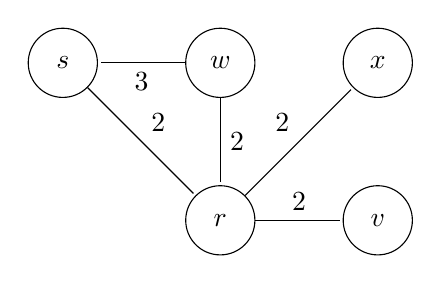
\begin{tikzpicture}[>=stealth',shorten >=1pt,auto,node distance=2cm]
  			\node[state]  (x) []           {$x$};
  			\node[state]             (w) [left of=x]  {$w$};
  			\node[state] 			 (s) [left of=w]  {$s$};
  			\node[state] 			 (r) [below of=w] {$r$};
  			\node[state]			 (v) [below of=x] {$v$};


  			\path[-] (w) edge node {2} (r)
        	         	 edge node {3} (s)
        	         (s) edge node {2} (r)
        	         (r) edge node {2} (v)
                     	 edge node {2} (x);
        	         
            	 		
		\end{tikzpicture}
	\end{center}
    
The minimum spanning tree of this graph is:  \\
\begin{center}
		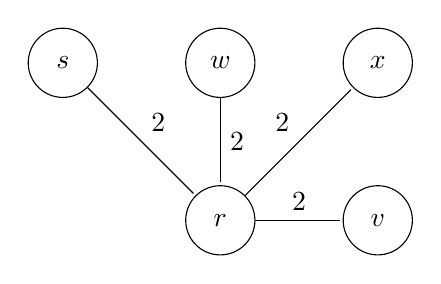
\begin{tikzpicture}[>=stealth',shorten >=1pt,auto,node distance=2cm]
  			\node[state]  (x) []           {$x$};
  			\node[state]             (w) [left of=x]  {$w$};
  			\node[state] 			 (s) [left of=w]  {$s$};
  			\node[state] 			 (r) [below of=w] {$r$};
  			\node[state]			 (v) [below of=x] {$v$};


  			\path[-] (w) edge node {2} (r)
        	         (s) edge node {2} (r)
        	         (r) edge node {2} (v)
                     	 edge node {2} (x);
        	         
            	 		
		\end{tikzpicture}
	\end{center}
The shortest path tree starting from s is: \\
\begin{center}
		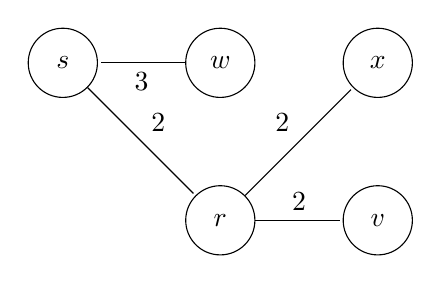
\begin{tikzpicture}[>=stealth',shorten >=1pt,auto,node distance=2cm]
  			\node[state]  (x) []           {$x$};
  			\node[state]             (w) [left of=x]  {$w$};
  			\node[state] 			 (s) [left of=w]  {$s$};
  			\node[state] 			 (r) [below of=w] {$r$};
  			\node[state]			 (v) [below of=x] {$v$};


  			\path[-] (w) edge node {3} (s)
        	         (s) edge node {2} (r)
        	         (r) edge node {2} (v)
                     	 edge node {2} (x);
        	         
            	 		
		\end{tikzpicture}
\end{center}

\end{document}